\section{Bipolare Transistoren (BJT)}

\renewcommand{\arraystretch}{1.3}
\begin{tabular}{|ll |ll|}
    \hline
    $I_E$   & Emitter-Strom     & $I_B$             & Basis-Strom                   \\
    \hline
    $I_C$   & Kollektor-Strom   & $\beta = h_{\rm FE}$  & Wechselstrom-Verstärkung  \\
    \hline
\end{tabular}
\renewcommand{\arraystretch}{1}


\subsection{Funktionsweise Bipolarer Transistor}

\begin{minipage}[c]{0.2\columnwidth}
    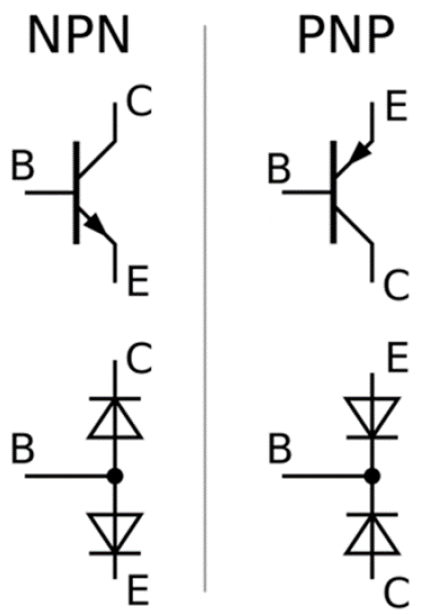
\includegraphics[width=\columnwidth]{images/BJT.png}
\end{minipage}
\hfill
\begin{minipage}[c]{0.78\columnwidth}
    \raggedright

    \begin{itemize}
        \item BK-Diode sperrt im Normalbetrieb
        \item BE-Diode leitet im Normalbetrieb \\
             \textbf{BJT ist nicht symmetrisch!}
        \item Hohe Dotierung im Emitter $(n^+)$
        \item Niedrige Dotierung im Kollektor ($n$, zum Anschluss hin $n^+$) \\
            \textrightarrow\ Kleiner Basis-Strom erzeugt grossen Kollektor-Strom
    \end{itemize}
\end{minipage}


\subsection{Bipolarer Transistor als Stromverstärker}

\begin{minipage}[c]{0.3\columnwidth}
    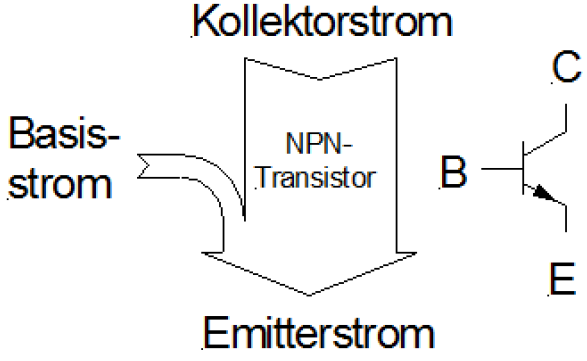
\includegraphics[width=\columnwidth]{images/BJT_funktionsweise.png}
\end{minipage}
\hfill
\begin{minipage}[c]{0.68\columnwidth}
    \renewcommand{\arraystretch}{1.4}
    \begin{tabular}{ll}
        $\boxed{ I_E = I_C + I_B }$         & Stromsummengleichung              \\
        $\boxed{ I_E \approx I_C} $         & vereinfacht für $\beta \gg 1 $    \\
        $\boxed{ I_C = \beta \cdot I_B}$    & 
    \end{tabular}
    \renewcommand{\arraystretch}{1}
\end{minipage}


\subsection{Betriebszustände des Transistors}

\begin{itemize}
    \item \textbf{Normalbetrieb} (forward region): $V_{\rm BE} > 0, \,  V_{BC} < 0$ \\
        E-Diode leitend, C-Diode sperrend. Es gilt: $\bm{I_C= \beta  \cdot I_B}$
    \item \textbf{Sättigung}: $V_{\rm BE} > 0, \,  V_{BC} > 0$ \\
        Beide Dioden leitend. \textbf{Schalter 'ON'}: $V_{\rm CE,sat}$ ca. $0.1..0.3 \, \volt$
    \item \textbf{Sperrbetrieb}: $V_{\rm BE} < 0, \,  V_{BC} < 0$ \\
        Beide Dioden sperrend. \textbf{Schalter 'OFF'}
    \item \textbf{Inversbetrieb}: $V_{\rm BE} < 0, \,  V_{BC} > 0$ \\
        Wie Normalbetrieb, aber nur wenig Stromverstärkung 
\end{itemize}


\subsection{Kennlinien}

\textbf{Im Arbeitsbereich wie Diode: } $ \bm{V_{\rm BE} = 0.7 \, \volt}$

\vspace{0.2cm}

\begin{minipage}[c]{0.33\columnwidth}
    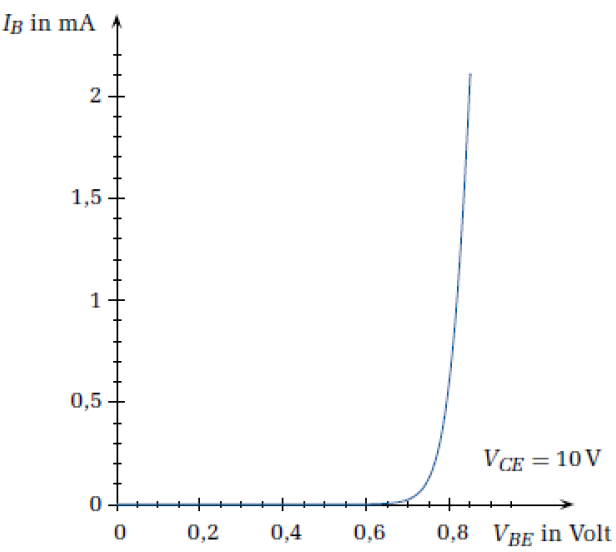
\includegraphics[width=\columnwidth]{images/BJT_eingangskennlinie.png}
\end{minipage}
\hfill
\begin{minipage}[c]{0.55\columnwidth}
    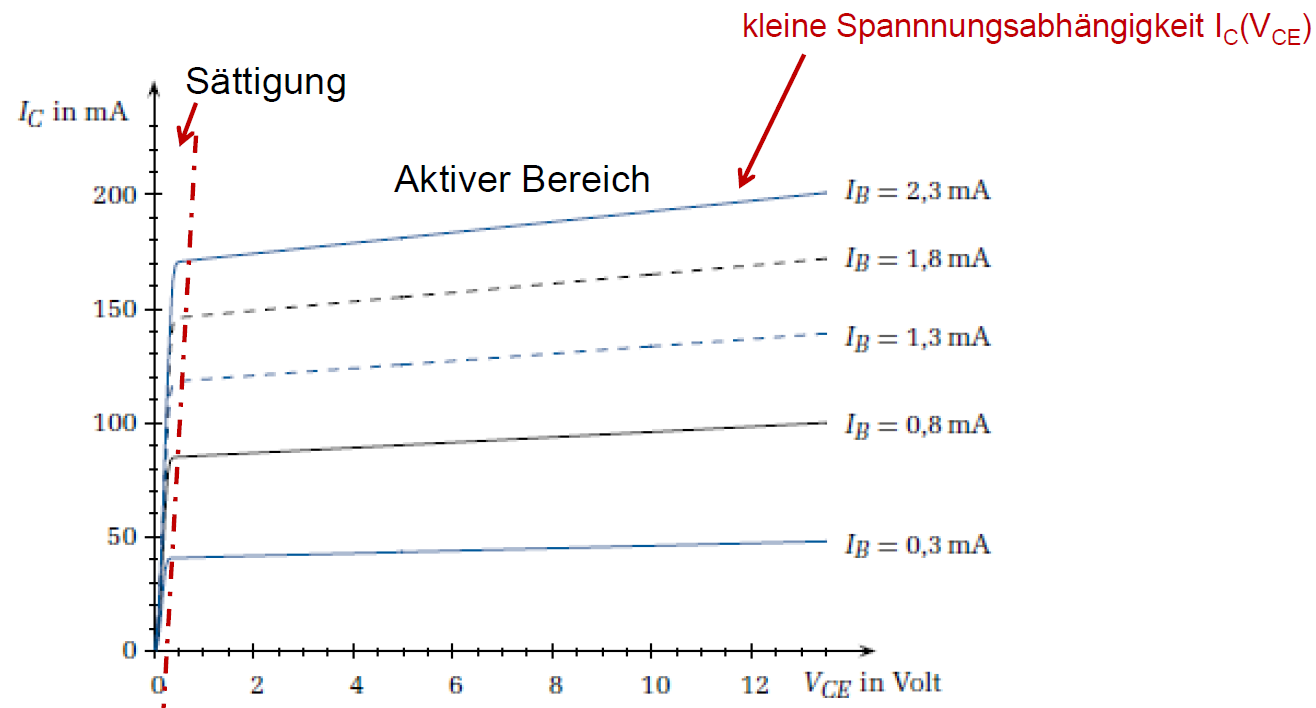
\includegraphics[width=\columnwidth]{images/BJT_ausgangskennlinien.png}
\end{minipage}


\subsection{Verlustleistung und Erwärmung im Transistor}

\vspace{-0.2cm}

$$ \boxed{ P_v = V_{\rm CE} \cdot (I_B + I_C) \approx  V_{\rm CE} \cdot I_C = V_{\rm AP} \cdot I_C } $$
$$ \boxed{ \Delta T = R_{\rm th} \cdot P_v }$$



\subsection{Ersatzschlatungen von Transistoren}

\subsubsection{Grosssignal-Ersatzschaltung}

\begin{minipage}[c]{0.48\columnwidth}
    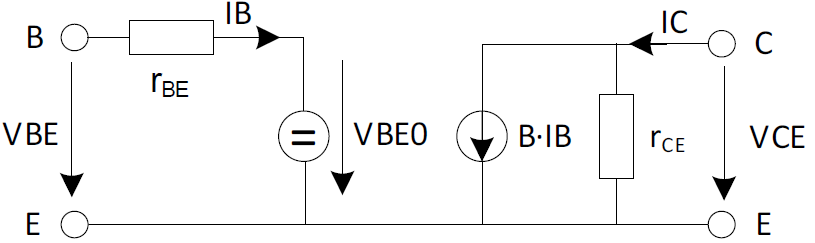
\includegraphics[width=\columnwidth]{images/BJT_grosssignalersatzschaltung.png}
\end{minipage}
\hfill
\begin{minipage}[c]{0.48\columnwidth}
    $$ \boxed{ R_{\rm BE} = \frac{n \cdot V_T}{I_{\rm B0}} } \qquad \boxed{ r_{\rm CE} \approx \frac{V_A}{I_C}} $$
\end{minipage}


\subsubsection{Kleinsignal-Ersatzschaltungen}

\begin{minipage}[c]{0.45\columnwidth}
    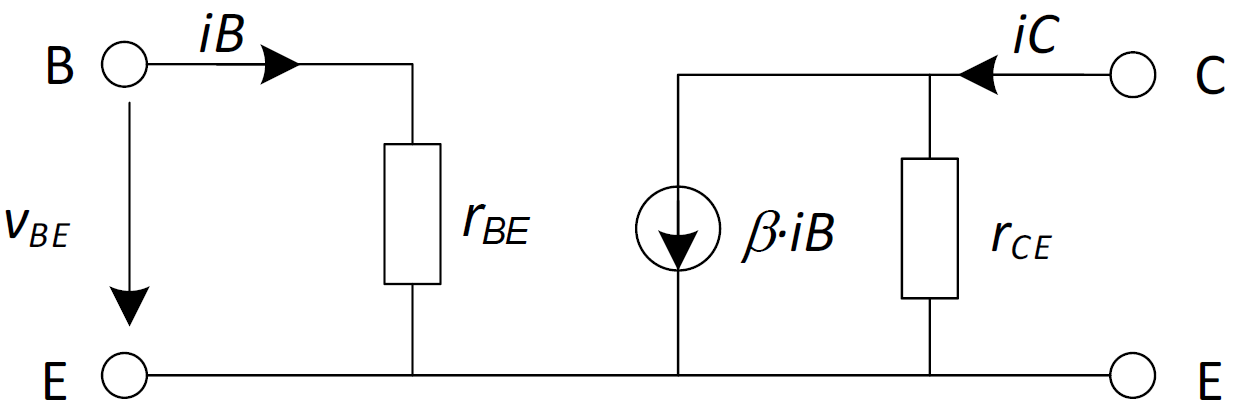
\includegraphics[width=\columnwidth]{images/BJT_kleinsignalmodell_1.png}
\end{minipage}
\hfill
\begin{minipage}[c]{0.45\columnwidth}
    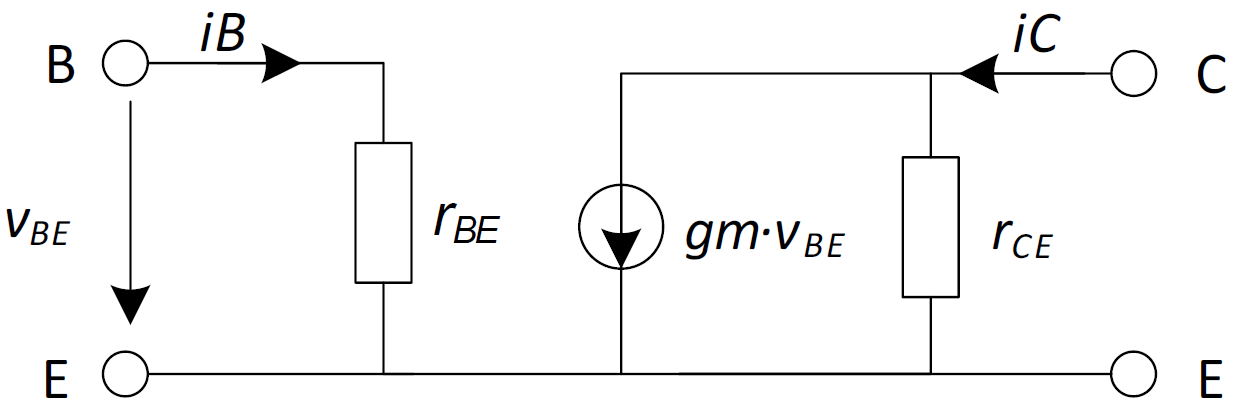
\includegraphics[width=\columnwidth]{images/BJT_kleinsignalmodell_2.png}
\end{minipage}

\vspace{0.2cm}

\begin{tabular}{@{}ccc@{}}
    $\boxed{ r_{\rm BE} = \frac{n \cdot V_T}{I_{\rm B0}} }$ & $\boxed{ gm = \frac{\beta}{r_{\rm BE}} = \frac{I_C}{n \cdot V_T} }$ & $\boxed{ r_{\rm CE} \approx \frac{V_A}{I_C} = \frac{200 \, \volt}{I_C} } \; V_A: \text{Early Spannung}$
\end{tabular}


\subsection{Emitterschaltung}

\begin{minipage}[c]{0.3\columnwidth}
    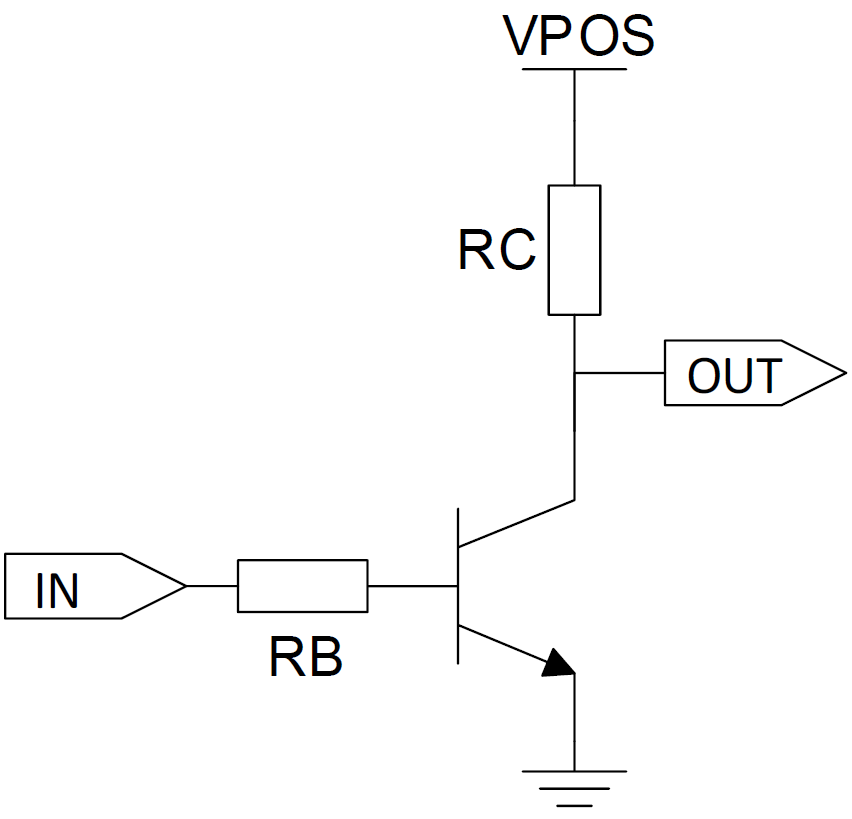
\includegraphics[width=0.8\columnwidth]{images/emitterschaltung_2.png}
    $$ \boxed{I_{\rm RC} = \frac{(V_{\rm POS} - V_{\rm out})}{R_C} } $$
\end{minipage}
\hfill
\begin{minipage}[c]{0.55\columnwidth}
    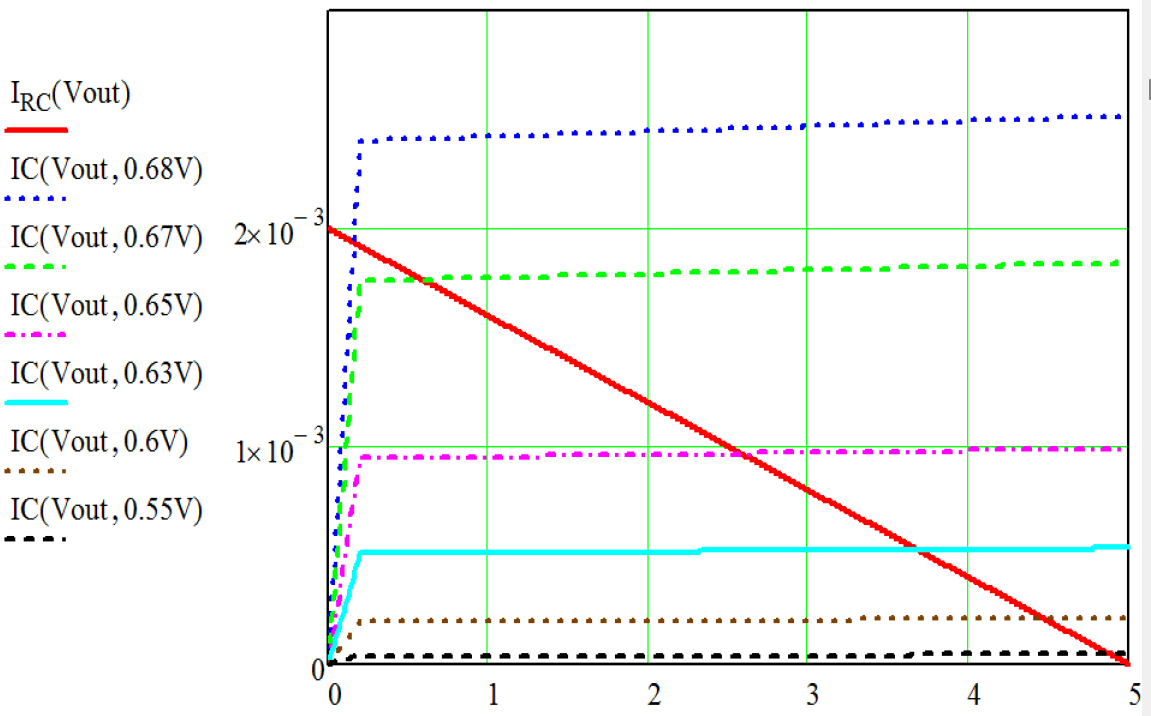
\includegraphics[width=\columnwidth]{images/emitterschaltung_kennlinienfeld.png}
\end{minipage}

\vspace{0.2cm}

\myul{\textbf{Arbeitsbereiche}}

\vspace{0.1cm}

\begin{tabular}{lll}
    Sperrend        & $ 0 \, \volt < V_{\rm BE} < ~0.6 \, \volt$ & $V_{\rm out} = V_{\rm POS}$                          \\
    Verstärkend     & $ \approx 0.6 \, \volt < V_{\rm BE} < ~0.8 \, \volt$ & $V_{\rm out}$ sinkt auf $V_{\rm CE,sat}$   \\
    Durchgesteuert  & $ \approx 0.8 \, \volt < V_{\rm BE}$ & $V_{\rm out} = V_{\rm CE,sat} $ 
\end{tabular}


\subsubsection{Emitterschaltung berechnen}

Gültig für $V_{\rm CE,sat} < V_{\rm out} < V_{\rm POS}$

\begin{minipage}[c]{0.7\columnwidth}
    $$ \boxed{ I_{\rm RC} = \frac{(V_{\rm POS} - V_{\rm out})}{R_C} = I_C = \beta \cdot I_S \cdot e^{\frac{V_{\rm in}}{n \cdot V_T}} } $$
    $$ \boxed{ V_{\rm out} = V_{\rm POS} - R_C \cdot \beta \cdot I_S \cdot e^{\frac{V_{\rm in}}{n \cdot V_T}} } $$
\end{minipage}
\begin{minipage}[c]{0.25\columnwidth}
    \[ \boxed{A = \frac{-R_c I_c}{n V_t}}\]
\end{minipage}

$V_{\rm out} = f(V_{\rm in})$ Exponentialfunktion: Start @ $V_{\rm POS}$, Ende @ $V_{\rm CE,sat}$


\subsection{Transistorverstärker mit Arbeitspunkteinstellung}

Spannung $V_{\rm out}$ soll auf $V_{AP}$ eingestellt werden: \\
$V_B$ entspricht Diodenspannung $\bm{ V_B = 0.7 \, V} $ 


\subsubsection{AP über Strom (bzw. $\bm{R_1}$) einstellen}

\begin{minipage}[c]{0.3\columnwidth}
    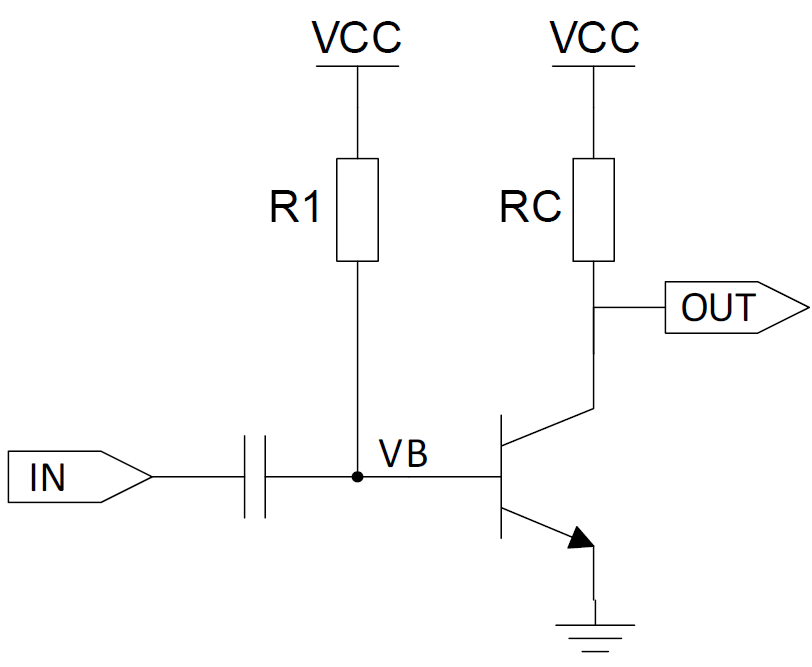
\includegraphics[width=\columnwidth]{images/emitterschaltung_AP_1.png}
\end{minipage}
\hfill
\begin{minipage}[c]{0.69\columnwidth}
    $$ \boxed{ I_{\rm C0} = \frac{V_{AP}}{R_C} } \quad \boxed{ I_{B0} = \frac{I_{\rm C0}}{\beta} } \quad \boxed{ R_1 = \frac{V_{CC} - V_B}{I_{B0}} } $$
\end{minipage}


\subsubsection{AP über Spannung (bzw. $\bm{R_1}$ und $\bm{R_2}$) einstellen}
\label{AP über Spannung (bzw. $R_1$ und $R_2$) einstellen}

\begin{minipage}[c]{0.3\columnwidth}
    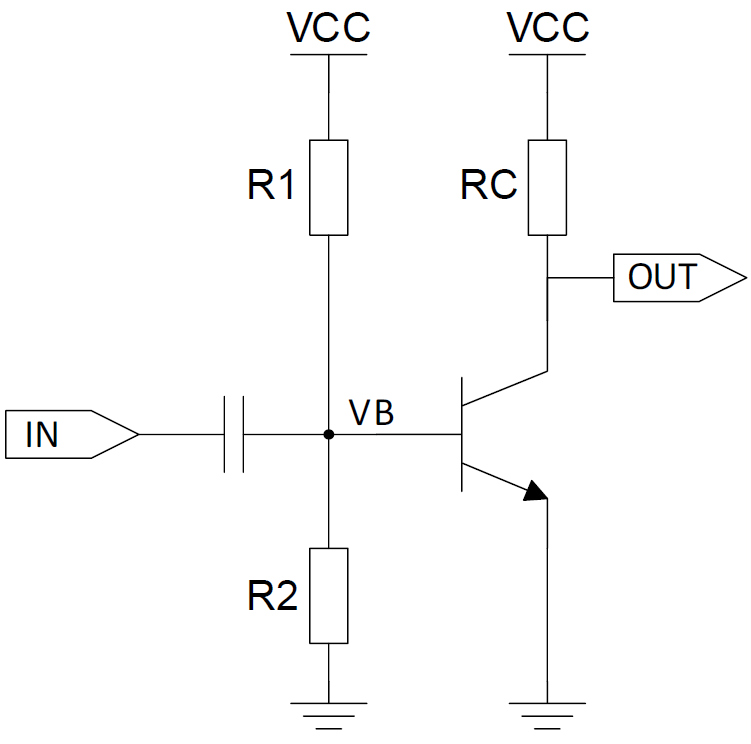
\includegraphics[width=\columnwidth]{images/emitterschaltung_AP_2.png}
\end{minipage}
\hfill
\begin{minipage}[c]{0.69\columnwidth}
    $$ \boxed{ I_{\rm C0} = \frac{V_{\rm AP}}{R_C} } \quad \boxed{ I_{\rm B0} = \frac{I_{\rm C0}}{\beta} } \quad \boxed{ I_{\rm R2} \geq 10 \cdot I_{\rm B0} } $$
    $$ \boxed{ R_2 = \frac{V_B}{I_{\rm R2}} } \quad \boxed{ R_1 = \frac{(V_{\rm CC} - V_B)}{I_{\rm B0} + I_{\rm R2}} } $$
\end{minipage}

\textrightarrow\ Schaltung hat sehr grosse Toleranzen! \\
\textrightarrow\ Temperatur-Abhägigkeit von $V_{\rm BE} = -2 \, \frac{\milli \volt}{\kelvin}$ \textrightarrow\ Faktor 2 alle $10 \, \celsius$ \\
\textrightarrow\ Somit ändern sich auch $I_B$ bzw. $I_C$ alle $10 \, \celsius$


\subsubsection{Transistorverstärker mit Stromgegenkopplung}

\begin{minipage}[c]{0.27\columnwidth}
    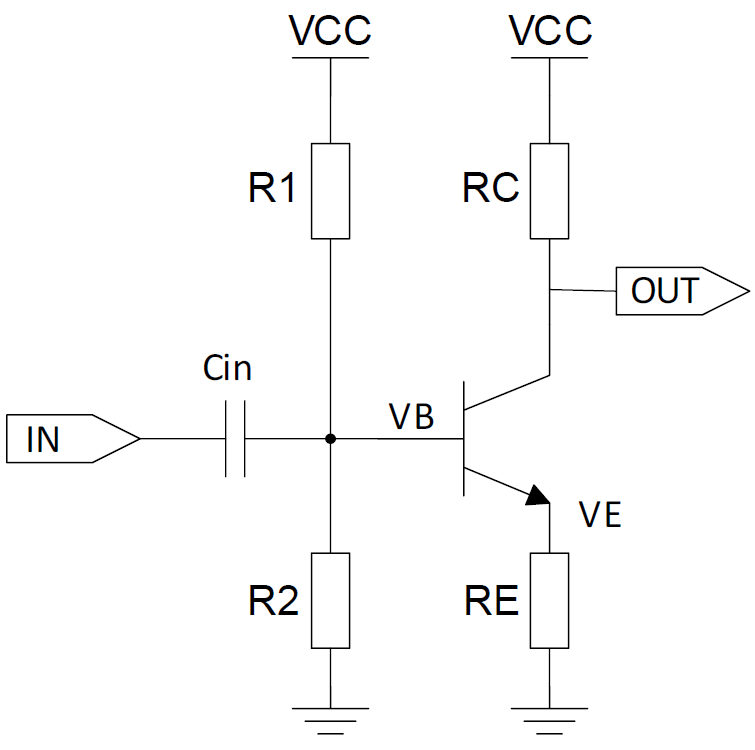
\includegraphics[width=\columnwidth]{images/transistorverstaerker_stromgegenkopplung.png}
\end{minipage}
\hfill
\begin{minipage}[c]{0.66\columnwidth}
    \raggedright
    \myul{\textbf{Reduktion der Toleranzen}}

    \vspace{0.1cm}

    $V_{\rm BE}$ entspricht Diodenspannung $\bm{ V_B = 0.7 \, V} $

    \vspace{0.2cm}
    $V_{\rm in}$ \textbf{steigt} um $\Delta V$ \\
    \textrightarrow\ Dann steigt auch $V_B$ um $\Delta V$ \\
    \textrightarrow\ Dann steigt auch $V_E$ um $\Delta V$
\end{minipage}

\vspace{0.2cm}

\renewcommand{\arraystretch}{1.2}
\begin{tabular}{ll}
    Strom in $R_E$ steigt:                      & $\Delta I_{\rm RE} = \frac{\Delta V_E}{R_E} \approx \frac{\Delta V_{\rm in}}{R_E}$    \\
    Strom in $R_C$ steigt:                      & $\Delta I_{\rm RC} = \frac{\Delta V_E}{R_E} \approx \frac{\Delta V_{\rm in}}{R_E}$    \\
    Spannung an $V_{\rm out}$ \textbf{sinkt}:   & $\Delta V_{\rm out} \approx - \frac{R_C}{R_E} \cdot \Delta V_{\rm in}$
\end{tabular}
\renewcommand{\arraystretch}{1}


\subsubsection{Transistorverstärker mit Stromgegenkopplung \& Kondi}

\begin{minipage}[c]{0.27\columnwidth}
    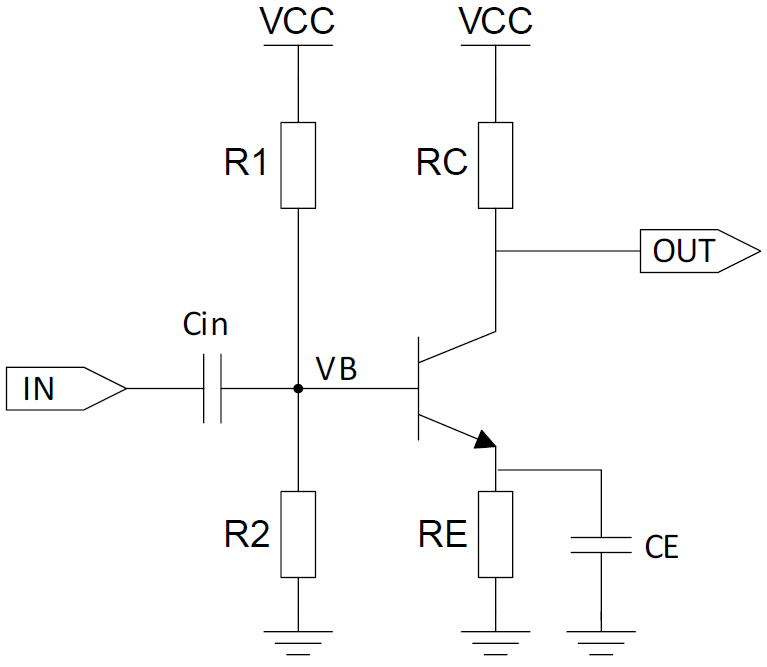
\includegraphics[width=\columnwidth]{images/transistorverstaerker_stromgegenkopplung_kondensator.png}
\end{minipage}
\hfill
\begin{minipage}[c]{0.66\columnwidth}
    $C_E$ schliesst $R_E$ für hohe Frequenzen kurz \\
    Somit wird der AP 'stabil' mit Widerständen eingestellt

    \vspace{0.2cm}

    Berechnung der Schaltung siehe Abschnitt \ref{AP über Spannung (bzw. $R_1$ und $R_2$) einstellen}
\end{minipage}


\subsection{Transistor als Schalter}

\begin{minipage}[c]{0.3\columnwidth}
    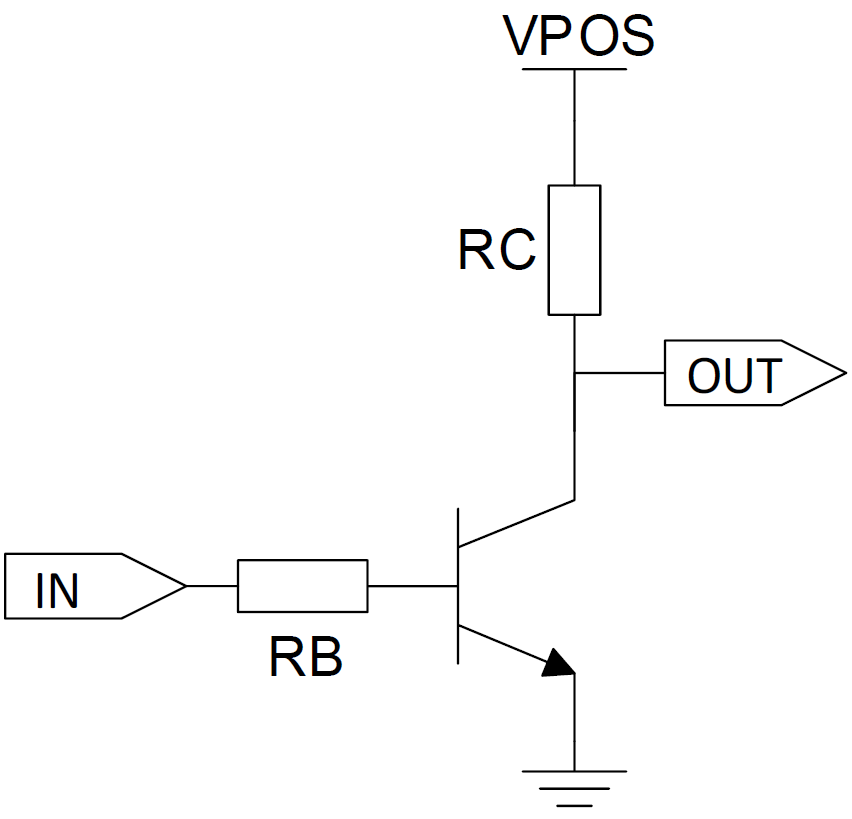
\includegraphics[width=\columnwidth]{images/emitterschaltung_2.png}
\end{minipage}
\hfill
\begin{minipage}[c]{0.46\columnwidth}
    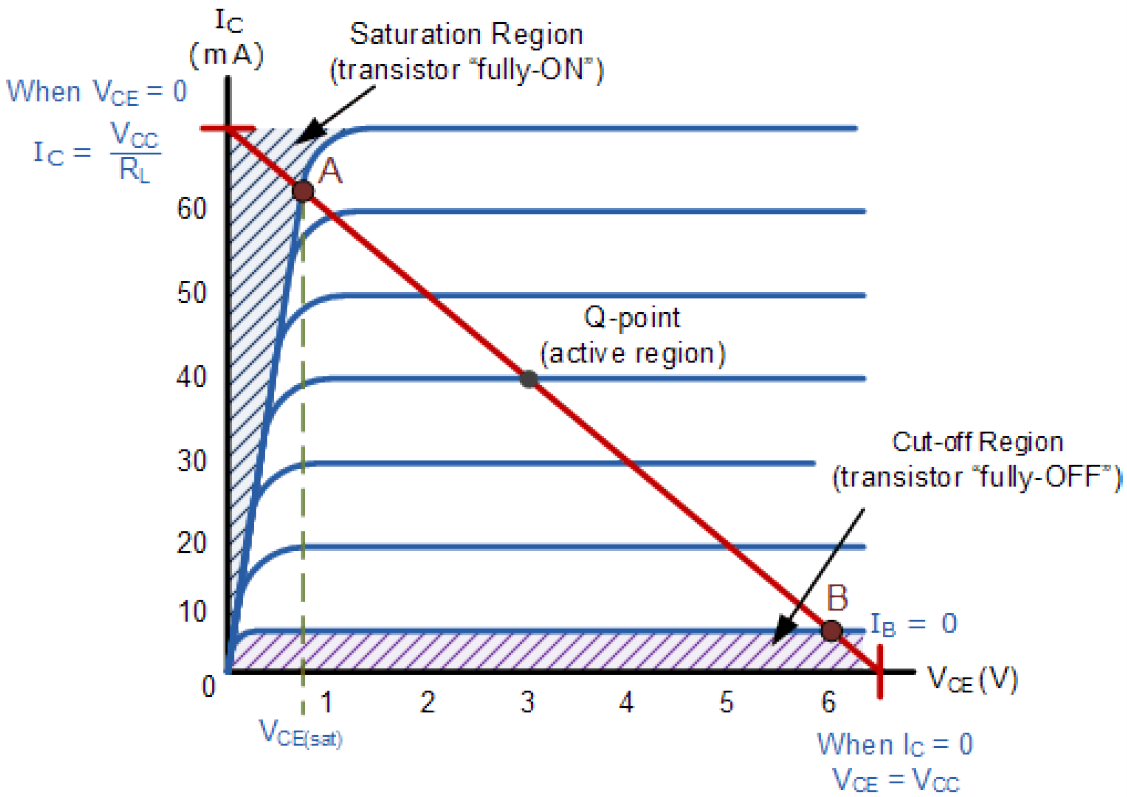
\includegraphics[width=\columnwidth]{images/transistor_als_schalter.png}
\end{minipage}

\vspace{0.2cm}

\begin{tabular}{lll}
    ON (A)  & $V_{\rm in} > 0.6$, grosses $I_B$ & \textrightarrow\ $V_{\rm out} = V_{\rm CE, sat}$  \\
    OFF (B) & $V_{\rm in} < 0.6 \, V$, $I_B = 0$ &  \textrightarrow\ $V_{\rm out} = V_{\rm CC}$
\end{tabular}


\subsection{Basisschaltung}

\subsubsection{Basischaltung als Verstärkerschaltung}

\begin{minipage}[c]{0.35\columnwidth}
$\bm{ V_{\rm BE0} = 0.7 \, V} $

\vspace{0.2cm}

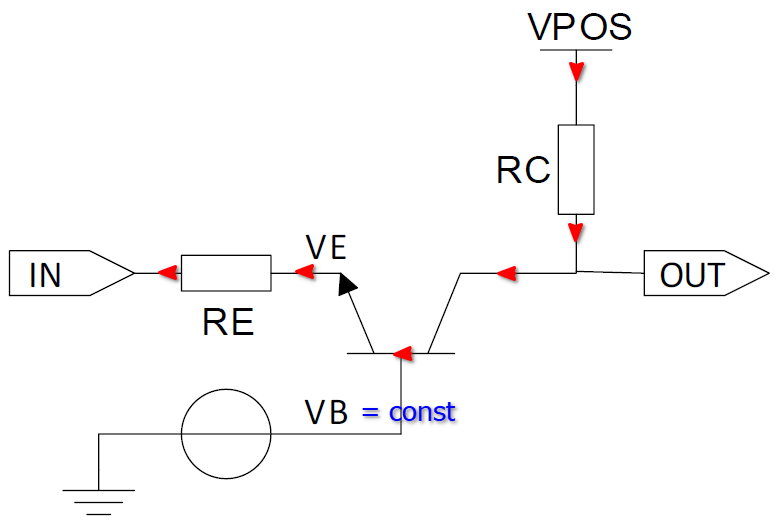
\includegraphics[width=\columnwidth]{images/basisschaltung_2}
\end{minipage}
\hfill
\begin{minipage}[c]{0.62\columnwidth}
    $$ \boxed{ I_E = I_C = \frac{(V_{\rm in} - V_{\rm BE0})}{R_E}  }$$
    $$ \boxed{ V_{\rm out} = V_{\rm POS} - I_E \cdot R_C - V_B}$$
    $$ \boxed{ \frac{\Delta V_{\rm out}}{\Delta V_{\rm in}} = \frac{R_C}{R_E} } \quad \boxed{ \Delta I = \frac{\Delta V_{\rm in}}{R_E}} $$
\end{minipage}

\vspace{0.2cm}

\myul{\textbf{Voraussetzungen:}}

\vspace{0.1cm}

\begin{tabular}{ll}
    $V_{\rm in} < V_B - V_{\rm BE0}$        & Strom fliesst aus Emitter     \\
    $V_{\rm out} > V_E + V_{\rm CE,sat}$    &                               \\
    $ V_B - V_{\rm BE0} + V_{\rm CE,sat}$   & Transtor als Verstärker       \\
    $I_B \approx 0$                         & \textrightarrow\ $I_E = I_C$
\end{tabular}


\subsubsection{Summierung von Bias- und Signalspannung}

\begin{minipage}[c]{0.35\columnwidth}
    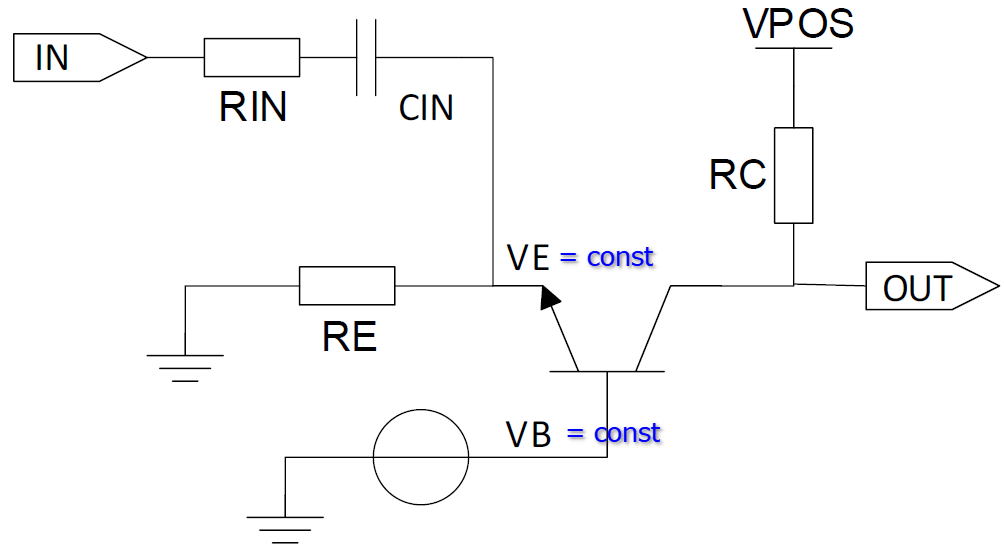
\includegraphics[width=\columnwidth]{images/basisschaltung_summierung.png}
\end{minipage}
\hfill
\begin{minipage}[c]{0.62\columnwidth}
    $\bm{ V_{\rm BE0} = 0.7 \, V} $

    $$ \boxed{ \Delta I_{\rm in} = \frac{\Delta V_{\rm in}}{R_{\rm in}} } \quad \boxed{ V_E = V_B - V_{\rm BE0} } $$
\end{minipage}

$$ \boxed{ V_{\rm out} = V_{\rm POS} - \Bigg( \frac{V_E}{R_E} - \frac{\Delta V_{\rm in}}{R_{\rm in}} \Bigg) \cdot R_C = V_{\rm out0} + \Delta V_{\rm in} \cdot \frac{R_C}{R_{\rm in}} } $$ 


\subsection{Kollektorschaltung (Emitterfolger)}

\begin{minipage}[c]{0.27\columnwidth}
    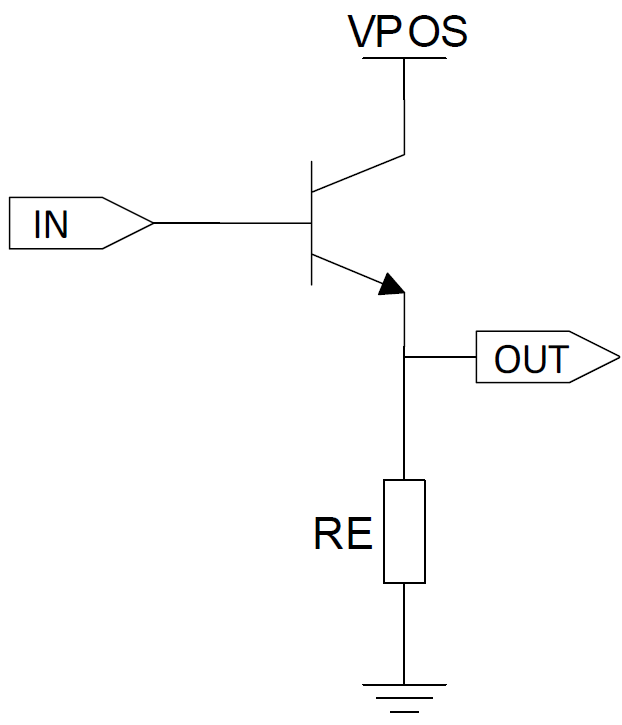
\includegraphics[width=\columnwidth]{images/kollektorschaltung_2.png}
\end{minipage}
\hfill
\begin{minipage}[c]{0.68\columnwidth}
    $$ \boxed{V_{\rm out} = V_{\rm in} - V_{\rm BE0} } $$
    $$ \boxed{ \text{Spannungsverstärkung } \approx 1 } $$

    \begin{itemize}
        \item Hoher Eingangswiderstand \\
            \textrightarrow\ $V_{\rm in}$ kaum belastet
        \item Tiefer Ausgangswiderstand \\
            \textrightarrow\ $V_{\rm out}$ kann Strom liefern 
    \end{itemize}
\end{minipage}


\subsection{Übresicht Verstärkertypen}

\begin{minipage}[c]{0.48\columnwidth}
    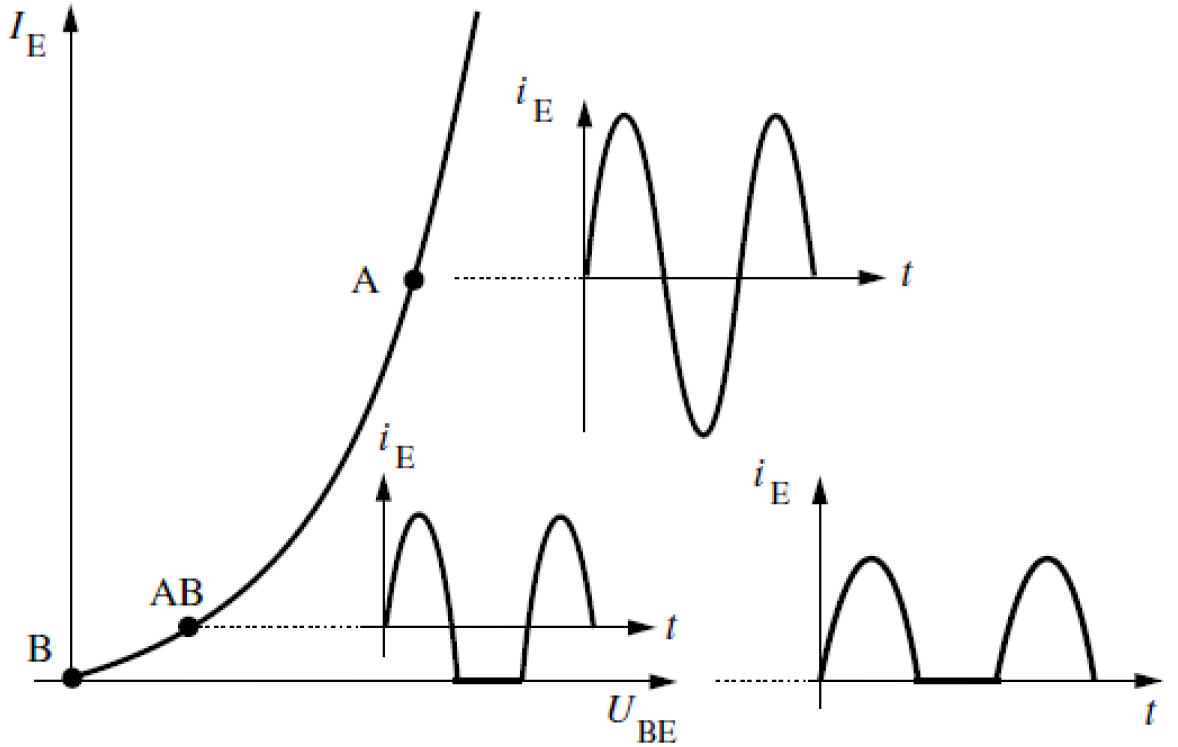
\includegraphics[width=\columnwidth]{images/verstaerker_uebersicht.png}
\end{minipage}
\hfill
\begin{minipage}[c]{0.48\columnwidth}
    \begin{tabular}{ll}
        A   & Einfacher Emitterfolger           \\
            & \textrightarrow\ sehr ineffizient \\
            & ($\eta_{\rm max} = 25$ \%)        \\
        B   & Effizient, aber verzerrt          \\
            & Signale um $0 \, V$               \\
            & ($\eta_{\rm max} = 78.5$ \%)      \\
        AB  & Guter Kompromiss für              \\
            & viele Anwendungen 
    \end{tabular}
\end{minipage}


\subsection{Class-A Verstärker}

\begin{minipage}[c]{0.3\columnwidth}
    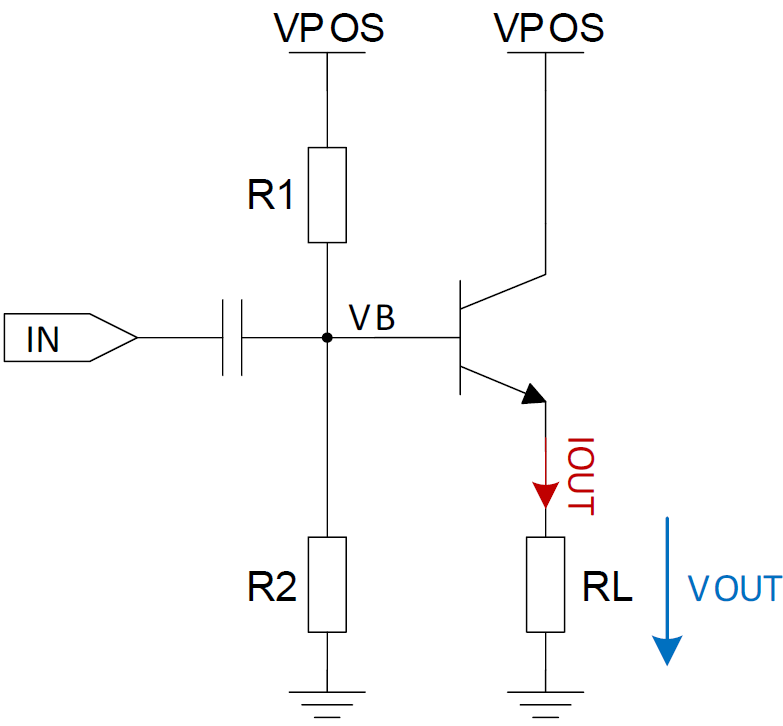
\includegraphics[width=\columnwidth]{images/class-A_verstaerker.png} 
\end{minipage}
\hfill
\begin{minipage}[c]{0.68\columnwidth}
    \raggedright
    $\bm{ V_{\rm BE0} = 0.7 \, V} $

    \vspace{0.2cm}

    \begin{itemize}
        \item $V_B$ eingestellt mit $R_1$ und $R_2$
        \item $V_B$ Es fliesst immer Strom durch $R_L$ \\
            \textrightarrow\ höheres $V_B$ \textrightarrow\ grösserer DC-Strom \\
            \textrightarrow\ grössere Verlustleistung
        \item wenn nicht 100\% ausgesteuert wird, nimt der Wirkungsgrad im Quadrat ab
    \end{itemize}
\end{minipage}


\subsubsection{Wirkungsgrad des Class-A Verstärkers}

$$ \boxed{ \eta \approx \frac{P_{\rm AC}}{P_{\rm DC} } \approx 25\%_{\text{MAX}}} \quad 
\boxed{P_{\rm AC} = V_{\rm eff} \cdot I_{\rm eff} = \frac{\hat{V}^2}{2 \cdot R_L}} \quad
\boxed{P_{\rm AC,MAX} =\frac{V_{\rm max}}{\sqrt{2}} \frac{\hat{I}_{\rm max}}{\sqrt{2}} = \frac{V_{\rm POS}^2}{8 R_L} } $$
$$ \boxed{ P_{\rm DC} = V_{\rm POS} \cdot I_L = V_{\rm POS} \cdot \frac{V_{\rm POS}}{2 \cdot R_L} = \frac{V_{\rm POS}^2}{2 \cdot R_L} } $$


\subsection{Class-B Verstärker}

\begin{minipage}[c]{0.3\columnwidth}
    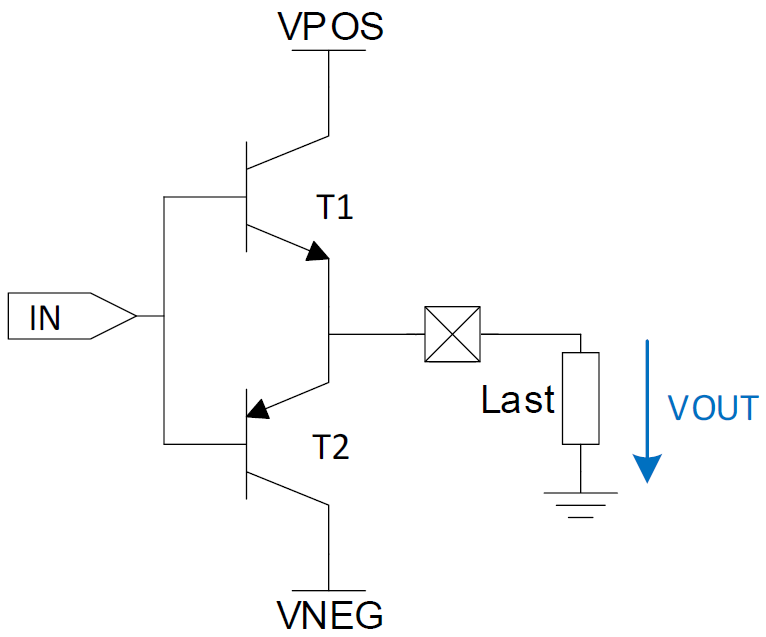
\includegraphics[width=\columnwidth]{images/class-B_verstaerker.png} 
\end{minipage}
\hfill
\begin{minipage}[c]{0.68\columnwidth}
    \raggedright

    \begin{itemize}
        \item $T1$ leitet für pos. Spannungen
        \item $T2$ leitet für neg. Spannungen \\
            \textrightarrow\ Es leiten nie beide Transistoren!
        \item Für $-0.7 \, V < V_{\rm in} < 0.7 \, V$ sperren beide Transistoren \\
            \textrightarrow\ \textbf{Verzerrungen} um $0 \, \volt$ 
    \end{itemize}
\end{minipage}


\subsubsection{Wirkungsgrad des Class-B Verstärkers}

\vspace{-0.2cm}

$$ \boxed{ \eta \approx \frac{P_{\rm AC}}{P_{\rm DC}} } \quad \boxed{ P_{\rm AC} = V_{\rm eff} \cdot I_{\rm eff} = \frac{\hat{V}^2}{2 \cdot R_L} } (\hat{V} \Rightarrow {\rm Spitzenwert})$$
$$ \boxed{ P_{\rm DC} = \frac{2}{T} \int\limits_0^{\frac{T}{2}}  V_{\rm POS} \cdot i(t) \, \diff t =
    \frac{2}{T} \int\limits_0^{\frac{T}{2}}  V_{\rm POS} \cdot \frac{V_{\rm max}}{R_L} \sin(x) \, \diff x = \frac{2}{\pi} \frac{V_{\rm POS} \cdot V_{\rm max}}{R_L} } $$


\subsection{Class-AB Verstärker}

\begin{minipage}[c]{0.3\columnwidth}
    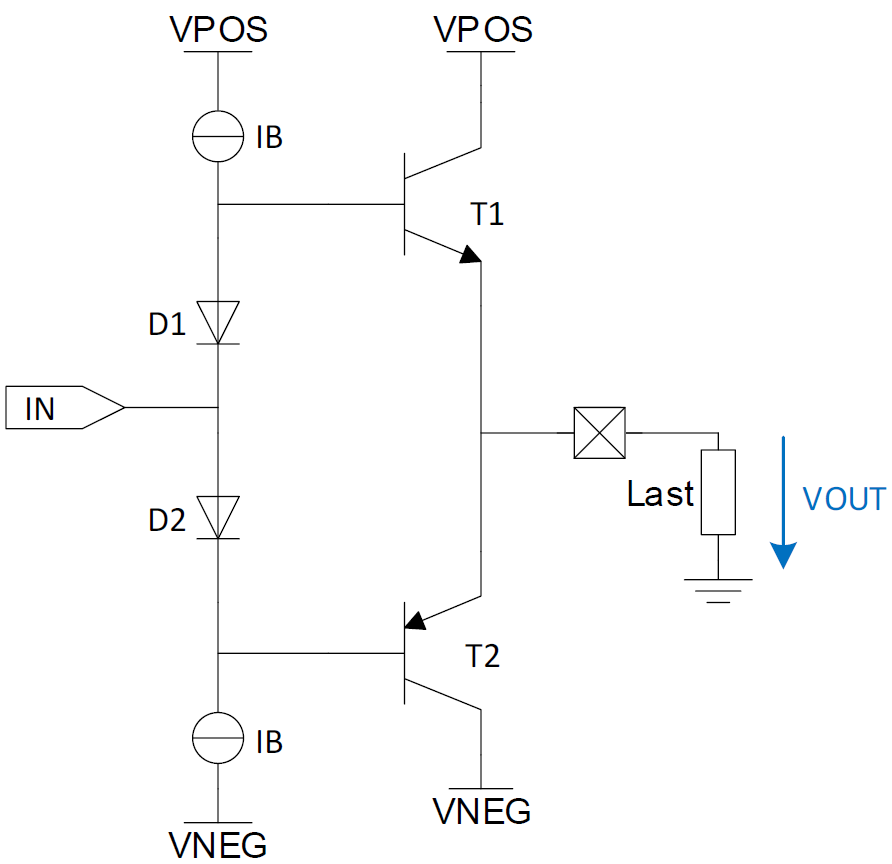
\includegraphics[width=\columnwidth]{images/class-AB_verstaerker.png} 
\end{minipage}
\hfill
\begin{minipage}[c]{0.68\columnwidth}
    \raggedright
    $\bm{ V_{\rm BE0} = 0.7 \, \volt} $

    \vspace{0.2cm}

    \begin{itemize}
        \item $D_1$: $T_1$ leitet für $V_{\rm in} > 0 \, \volt$
        \item $D_2$: $T_2$ leitet für $V_{\rm in} < 0 \, \volt$
        \item Einer der Transistoren leitet immer \\
            \textrightarrow\ Im Übergangsbereich leiten beide wenig
        \item $I_B$ liefern Basis- und Diodenströme 
    \end{itemize}
\end{minipage}


\subsubsection{Bipolar-Transistor mit $\bm{V_{\rm BE} = V_{\rm CE}}$}

\begin{minipage}[c]{0.2\columnwidth}
    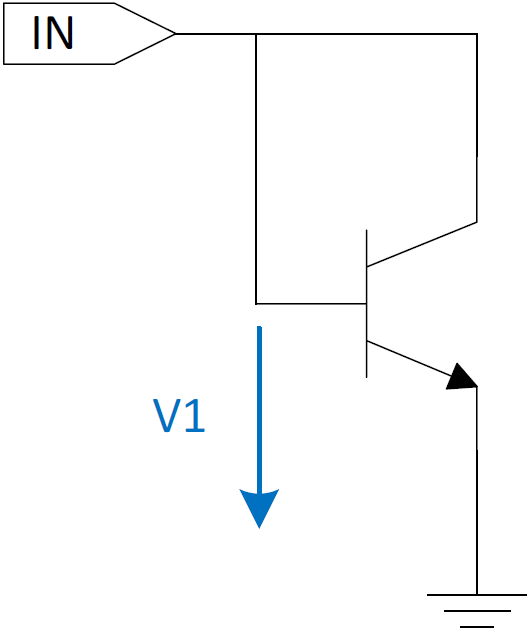
\includegraphics[width=\columnwidth]{images/BJT_VBE_VCE.png}
\end{minipage}
\hfill
\begin{minipage}[c]{0.2\columnwidth}
    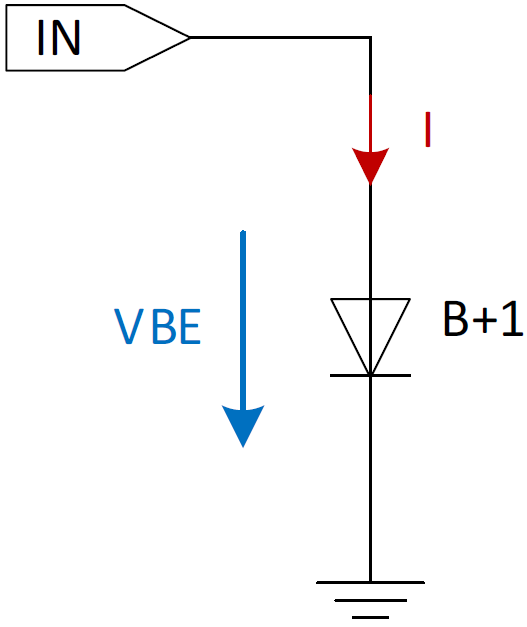
\includegraphics[width=\columnwidth]{images/BJT_parallele_dioden.png}
\end{minipage}
\hfill
\begin{minipage}[c]{0.2\columnwidth}
    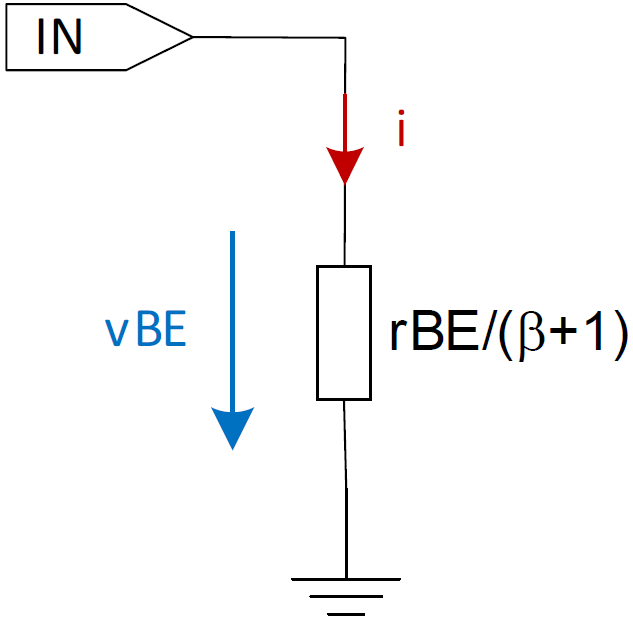
\includegraphics[width=\columnwidth]{images/BJT_kleinsignalersatzschaltung.png}
\end{minipage}
\hfill
\begin{minipage}[c]{0.3\columnwidth}
    $$ \boxed{r_{\rm BE} = \frac{n \cdot V_T}{I_{\rm B0}} } $$
    $$ \boxed{r_{\rm d,eq} = \frac{n \cdot V_T}{I_{\rm C0}} } $$
\end{minipage}


\subsection{Stromspiegel}

\begin{minipage}[c]{0.35\columnwidth}
    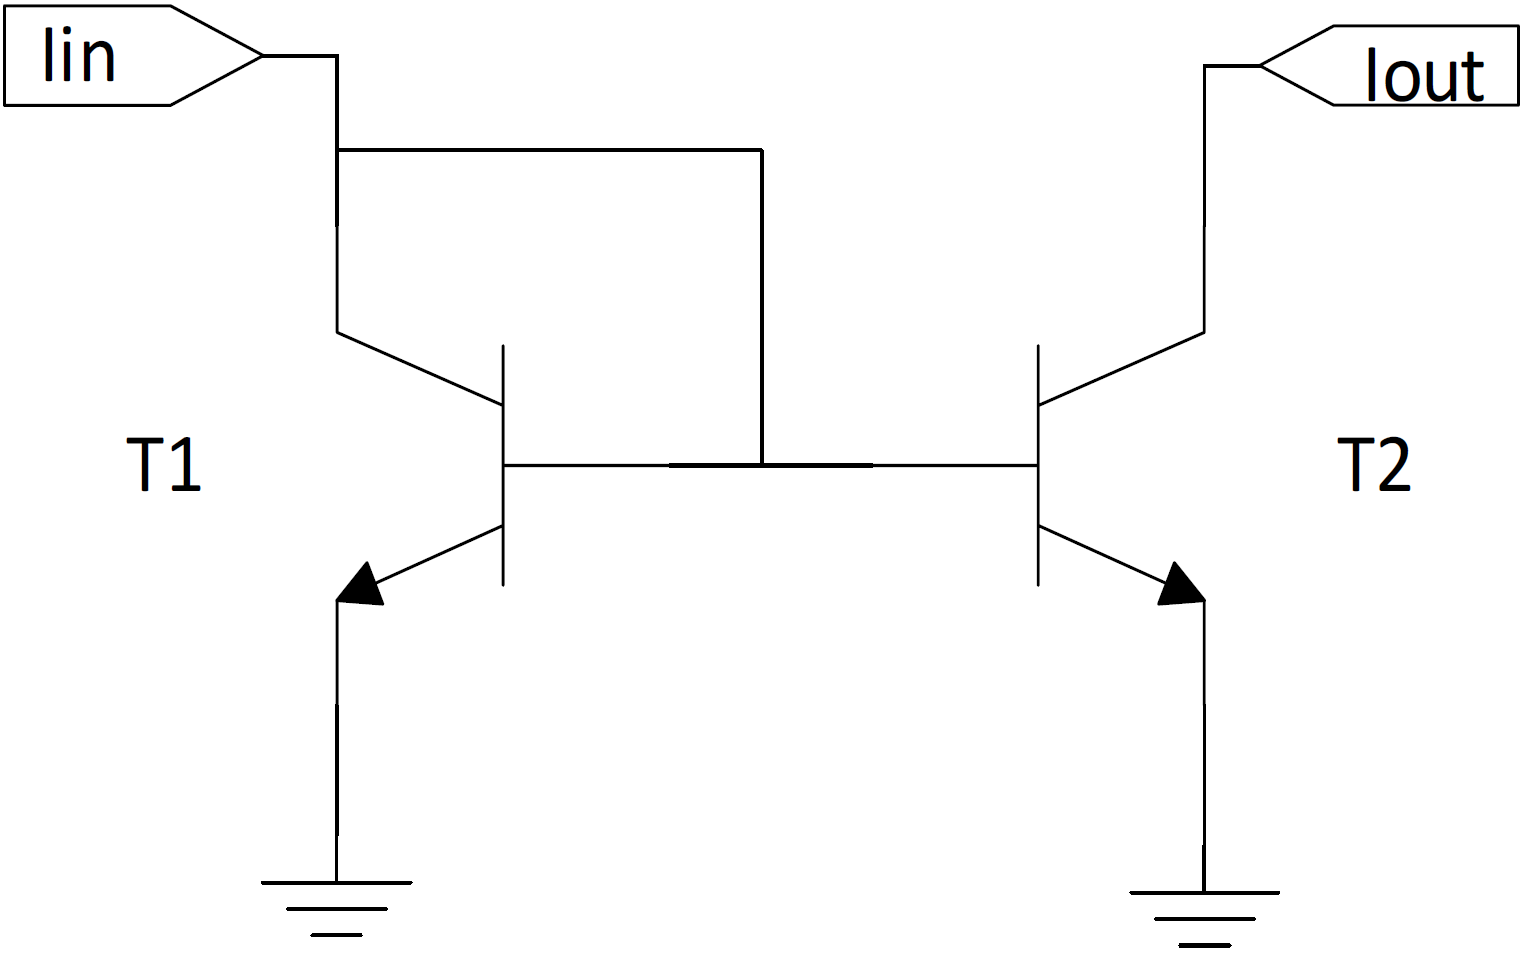
\includegraphics[width=\columnwidth]{images/stromspiegel.png}
\end{minipage}
\hfill
\begin{minipage}[c]{0.63\columnwidth}
    \begin{center}
        \begin{itemize}
            \item $T_1$ als Diode geschaltet
            \item $T_2$ hat gleiches $V_{\rm BE}$
            \item $V_{\rm BE,1} = V_{BE,2}$ \textrightarrow\ $I_{\rm B1} = I_{\rm B2}$ \\
                \textrightarrow\ $I_{\rm C1} = I_{\rm C2}$ 
        \end{itemize}
    
        $$ \boxed{ I_{\rm out} = I_{\rm in}} $$
    \end{center}
\end{minipage}


\subsubsection{Widlar-Stromspiegel}

\begin{minipage}[c]{0.3\columnwidth}
    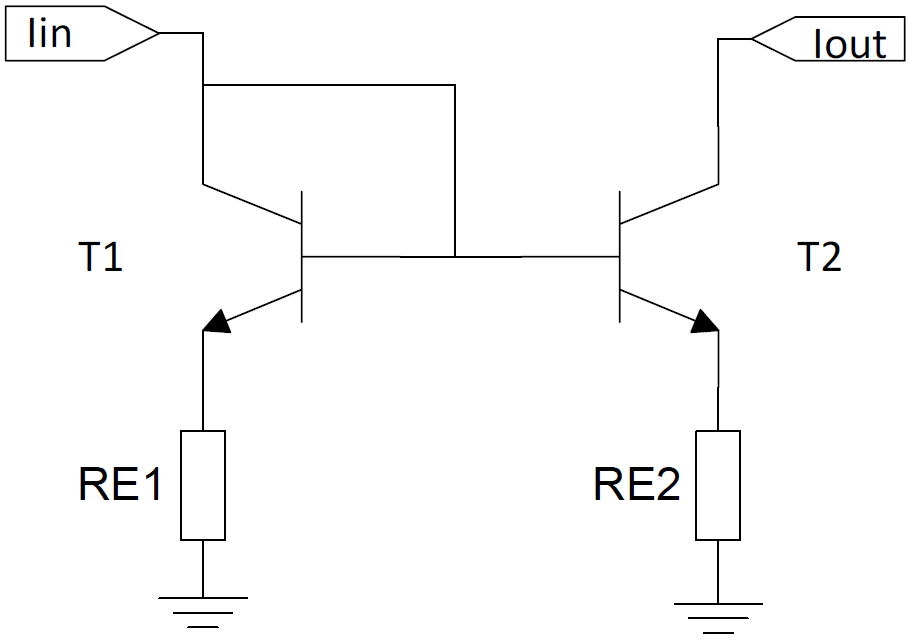
\includegraphics[width=\columnwidth]{images/widlar_stromspiegel.png}
\end{minipage}
\hfill
\begin{minipage}[c]{0.63\columnwidth}
    $$ \boxed{I_{\rm out} = I_{\rm in} \frac{R_{\rm E1}}{R_{\rm E2}} } $$
\end{minipage}


\subsubsection{Stromspiegel mit Kaskode}

\begin{minipage}[c]{0.28\columnwidth}
    \begin{center}
        \myul{\textbf{Stromspiegel}}

        \vspace{0.1cm}

        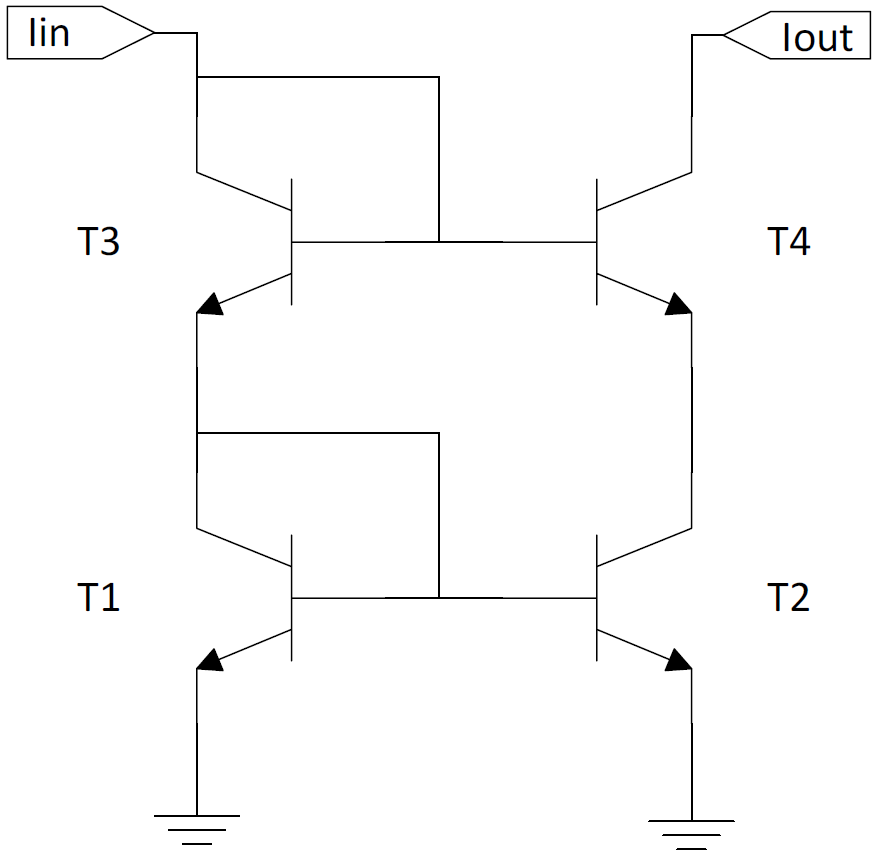
\includegraphics[width=\columnwidth]{images/kaskode.png}
    \end{center}
\end{minipage}
\hfill
\begin{minipage}[c]{0.28\columnwidth}
    \begin{center}
        \myul{\textbf{Funktionsweise}}

        \vspace{0.1cm}

        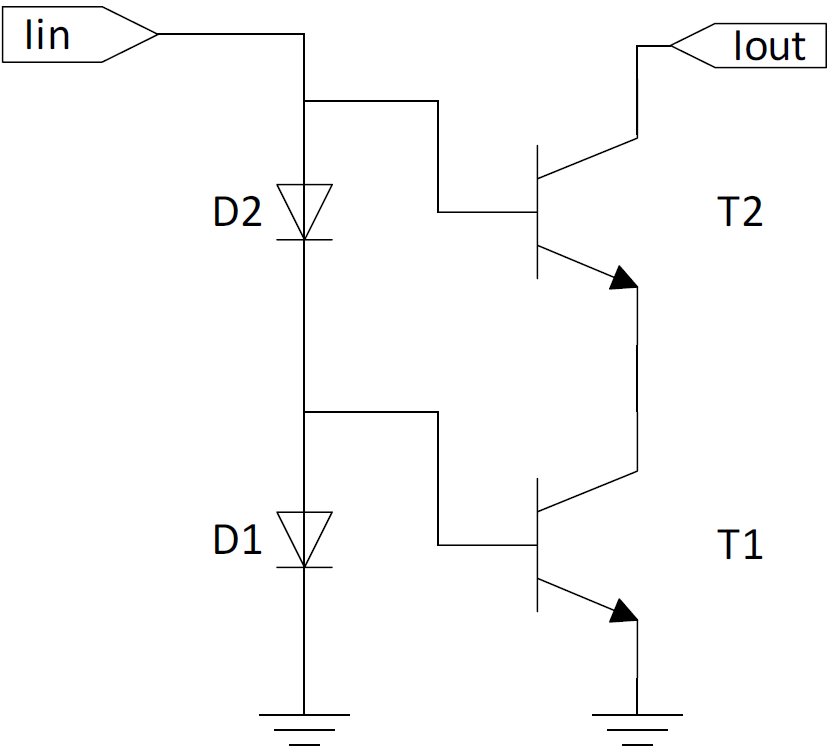
\includegraphics[width=\columnwidth]{images/kaskode_funktionsweise.png}
    \end{center}
\end{minipage}
\hfill
\begin{minipage}[c]{0.4\columnwidth}
    \begin{tabular}{ll@{}}
        $I_{\rm out}$   & Entspricht Kollektorstrom                        \\
                        & von $T_4$                                         \\
        $T_1$           & Als Diode beschaltet                              \\ 
                        & \textrightarrow\ $V_{\rm BE,1} = V_{\rm BE,2}$    \\
                        & \textrightarrow\ $IC_{\rm T1} = IC_{\rm T2}$      \\
        $T_3$           & Als Diode beschaltet                              \\
                        & \textrightarrow\ $V_{\rm CE,2} = 0.7 \, \volt$    \\
        $T_4$           & In Basisschaltung 
        \end{tabular}
\end{minipage}


\subsection{Differenzverstärker}

Differenzverstärker werden als Eingangsstufen von OpAmps oder Highest Speed Logik (LVDS, CML, ECL) eingesetzt. 


\subsubsection{Transistorpaar mit Emitterspannungen $\bm{V_E = 0 \, \volt}$}

\begin{minipage}[c]{0.35\columnwidth}
    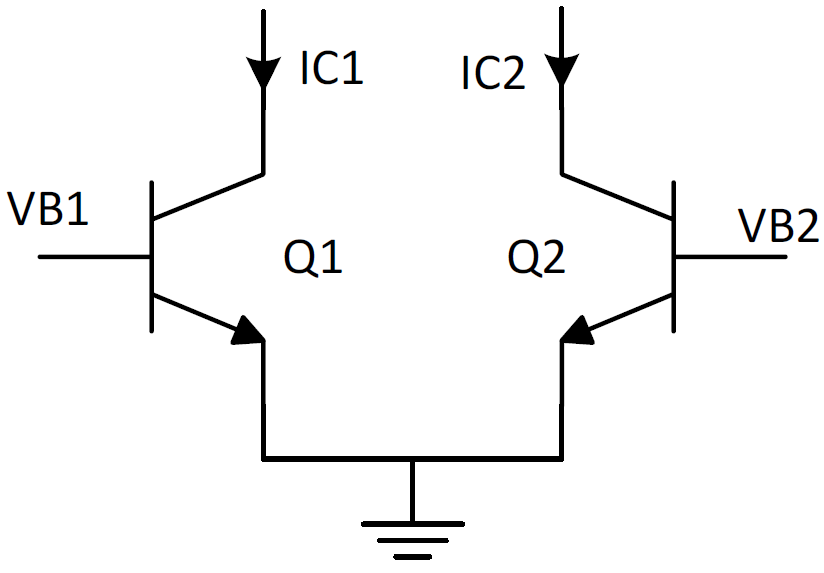
\includegraphics[width=\columnwidth]{images/transistorpaar.png}
\end{minipage}
\hfill
\begin{minipage}[c]{0.6\columnwidth}
    \raggedright
    Kleines $\Delta V$ führt zu grossem $\Delta I$
    
    \vspace{0.2cm}

    \begin{itemize}
        \item $V_{\rm B1} = V_{\rm BE0} + V_D = 0.7 \, \volt + V_D$
        \item $V_{\rm B2} = V_{\rm BE0}$ 
    \end{itemize}

    $$ \boxed{ \frac{I_{\rm C1}}{I_{\rm C2}} =  \frac{I_C ( V_{\rm BE0} + V_D)}{I_C (V_{\rm BE0} ) } = e^{\frac{V_D}{n \cdot V_T}} } $$
\end{minipage}


\subsubsection{Differenzstufe mit Stromquelle $\bm{I_{\rm BIAS}}$}

\begin{minipage}[c]{0.35\columnwidth}
    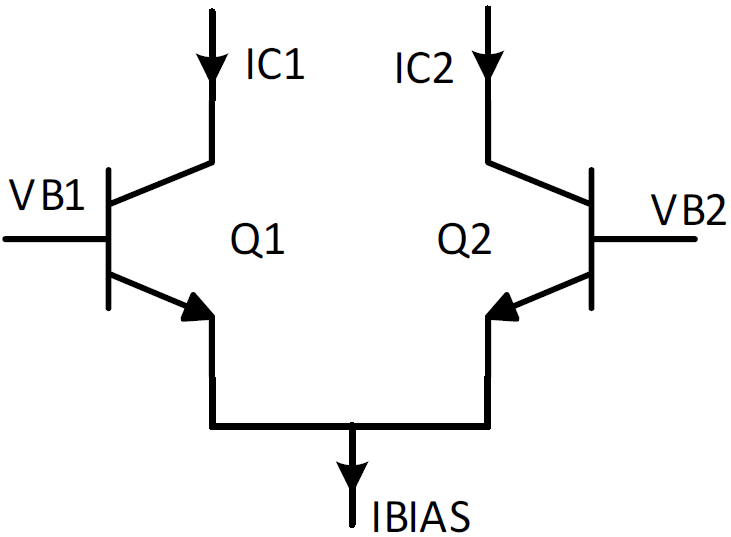
\includegraphics[width=\columnwidth]{images/differenzstufe_IBIAS.png}
\end{minipage}
\hfill
\begin{minipage}[c]{0.6\columnwidth}
    \raggedright

    \begin{itemize}
        \item $I_{\rm BIAS} = I_{\rm C1} + I_{\rm C2} = \const$
        \item $V_{\rm BE2} = V_{\rm B2} - V_E$
        \item $V_{\rm BE1} = V_{\rm BE2} + V_D$
    \end{itemize}

    $$ \boxed{ I_{\rm C1} = \beta \cdot I_S \cdot e^{\frac{V_{\rm BE2} + V_D}{n \cdot V_T}} = I_{\rm C2} \cdot e^{\frac{V_D}{n \cdot V_T}} } $$
    $$ \boxed{ I_{\rm BIAS} \approx I_{\rm C1} + I_{\rm C2} = I_{\rm C2} \cdot ( e^{\frac{V_D}{n \cdot V_T}} + 1) } $$
\end{minipage}


\subsubsection{Differenzstufe mit Stromquelle \& Kollektorwiderstand}

\begin{minipage}[c]{0.4\columnwidth}
    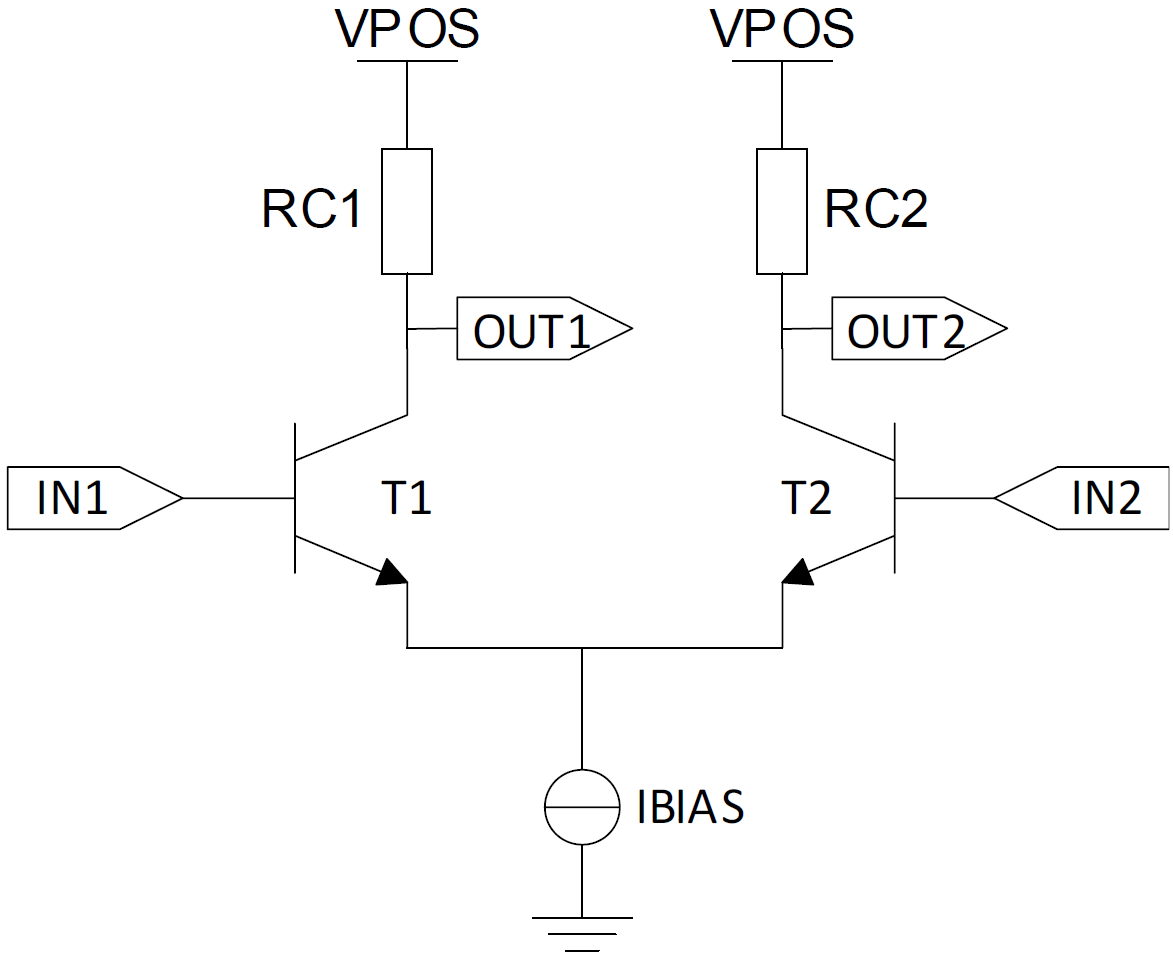
\includegraphics[width=\columnwidth]{images/differenzstufe_kollektorwiderstand.png}
\end{minipage}
\hfill
\begin{minipage}[c]{0.55\columnwidth}
    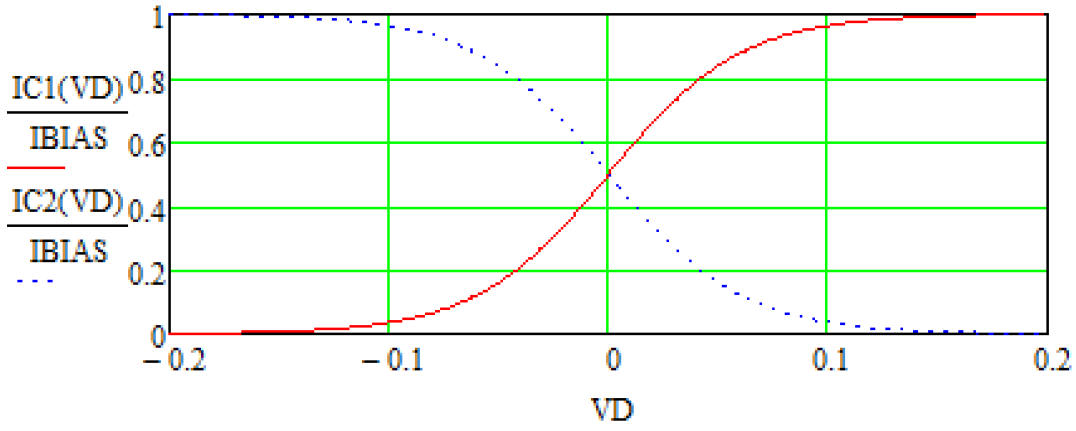
\includegraphics[width=\columnwidth]{images/differenzstufe_kollektorwiderstand_strom.png}
\end{minipage}

\vspace{0.2cm}

\begin{itemize}
    \item $V_D = 0$ durch beide Transistoren fliesst $\frac{I_{\rm BIAS}}{2}$
    \item $|V_D| = 200 \, \milli \volt$ ganzer Strom durch einen Transistor
    \item Im Bereich $\pm 100 \, \milli \volt$ teilt sich Strom auf
    \item $|V_D| < 200 \, \milli \volt$ $V_{\rm out} = V_{\rm out,0} + A \cdot \Delta V_{\rm in}$ \\
        $V_{\rm out,0}$ entspricht Ausgangsspannung @ $V_{\rm in1} = V_{\rm in2} $
\end{itemize}

\columnbreak

